\documentclass[border=8pt]{standalone}
\usepackage{amsmath}
\usepackage{amssymb}
\usepackage{tikz}
\usetikzlibrary{arrows.meta,calc,decorations.pathreplacing,patterns,shapes.geometric,positioning,shadings,plotmarks}

\begin{document}
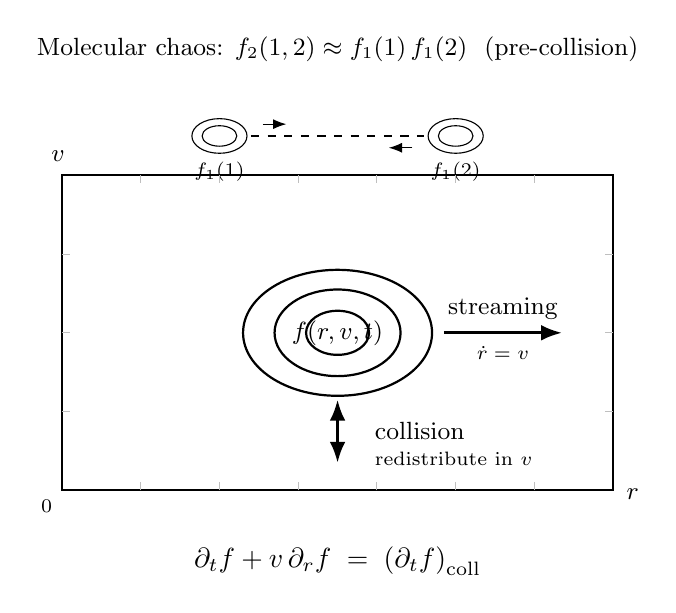
\begin{tikzpicture}[
    >=Latex,
    every node/.style={font=\small},
    contour/.style={thick, black},
    streamarr/.style={->, line width=1pt, black},
    collarr/.style={<->, line width=1pt, black},
    smallcontour/.style={thin, black}
]

% Top label: Stosszahlansatz
\node[align=center, font=\small] at (3.5, 5.6)
  {Molecular chaos: $f_2(1,2)\approx f_1(1)\,f_1(2)$ \ (pre-collision)};

% Two small contour blobs above (pre-collision pair)
\begin{scope}[shift={(2.0, 4.5)}]
  \draw[smallcontour] (0,0) ellipse (0.35 and 0.22);
  \draw[smallcontour] (0,0) ellipse (0.22 and 0.13);
  \node[font=\scriptsize] at (0, -0.45) {$f_1(1)$};
\end{scope}

\begin{scope}[shift={(5.0, 4.5)}]
  \draw[smallcontour] (0,0) ellipse (0.35 and 0.22);
  \draw[smallcontour] (0,0) ellipse (0.22 and 0.13);
  \node[font=\scriptsize] at (0, -0.45) {$f_1(2)$};
\end{scope}

% Dashed line connecting the pair (independent before collision)
\draw[dashed, thin] (2.4, 4.5) -- (4.6, 4.5);
\draw[->, thin] (2.55, 4.65) -- (2.85, 4.65);
\draw[->, thin] (4.45, 4.35) -- (4.15, 4.35);

% Phase space frame: rectangle with axes r (horizontal) and v (vertical)
\draw[thick] (0, 0) rectangle (7, 4);

% Axis labels
\node[font=\small] at (7.25, -0.05) {$r$};
\node[font=\small] at (-0.05, 4.25) {$v$};

% Tick marks (light grid feel)
\foreach \x in {1, 2, 3, 4, 5, 6} {
  \draw[gray!50, thin] (\x, 0) -- (\x, 0.1);
  \draw[gray!50, thin] (\x, 4) -- (\x, 3.9);
}
\foreach \y in {1, 2, 3} {
  \draw[gray!50, thin] (0, \y) -- (0.1, \y);
  \draw[gray!50, thin] (7, \y) -- (6.9, \y);
}

% Origin tick
\node[font=\scriptsize, anchor=north east] at (0, 0) {$0$};

% Central f(r,v,t) blob: 3 concentric ellipses
\begin{scope}[shift={(3.5, 2.0)}]
  \draw[contour] (0, 0) ellipse (1.2 and 0.8);
  \draw[contour] (0, 0) ellipse (0.8 and 0.55);
  \draw[contour] (0, 0) ellipse (0.4 and 0.28);
  \node[font=\small] at (0, 0) {$f(r,v,t)$};
\end{scope}

% Streaming arrow: horizontal, to the right of the blob
\draw[streamarr] (4.85, 2.0) -- (6.35, 2.0);
\node[font=\small, anchor=south, align=center] at (5.6, 2.05)
  {streaming};
\node[font=\scriptsize, anchor=north] at (5.6, 1.95)
  {$\dot r = v$};

% Collision arrow: vertical double-headed, below the blob
\draw[collarr] (3.5, 0.35) -- (3.5, 1.15);
\node[font=\small, anchor=west, align=left] at (3.85, 0.75)
  {collision};
\node[font=\scriptsize, anchor=west] at (3.85, 0.40)
  {redistribute in $v$};

% Bottom equation
\node[align=center, font=\normalsize] at (3.5, -0.9)
  {$\partial_t f + v\,\partial_r f \;=\; \left(\partial_t f\right)_{\mathrm{coll}}$};

\end{tikzpicture}
\end{document}
